% +------------------------------------------------------------------------+
% | CGAL Reference Manual:  Subdivision_method_3
% +------------------------------------------------------------------------+
% | Subdivision surfaces.
% | 
% | 1.2.2005  Le-Jeng Andy Shiue
% |
\RCSdef{\subdivisionRev}{$Id$}
\RCSdefDate{\subdivisionDate}{$Date$}
% +------------------------------------------------------------------------+

\ccParDims

\chapter{3D Surface Subdivision Methods}
\label{chapterSubdivision}
\ccChapterRelease{\subdivisionRev. \ \subdivisionDate}
\ccChapterAuthor{Le-Jeng Andy Shiue}
\hspace{.4cm}
\begin{ccTexOnly}
    \setlength{\unitlength}{1mm}
    \begin{picture}(0,0)(0.0,0.0)
      \put (78,25){% textwidth = 156mm
          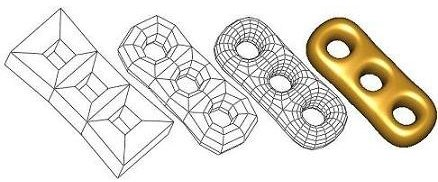
\includegraphics[width=0.5\textwidth]{Subdivision_method_3/FIG/teaser}
      }
    \end{picture}\vspace{-4mm}% compensate for some vspace added by picture
\end{ccTexOnly}

\minitoc

% +------------------------------------------------------------------------+
\section{Introduction} \label{sectionSubIntro}
% +------------------------------------------------------------------------+
Subdivision methods are simple yet powerful ways to 
generate smooth surfaces from arbitrary polyhedral meshes. 
Unlike spline-based surfaces (e.g NURBS) or other numeric-based 
modeling techniques, users of subdivision
methods do not need the mathematical knowledge of 
the subdivision methods. 
The natural intuition of the geometry suffices to control the 
subdivision methods. 

%Subdivision algorithms (see e.g.~\cite{cgal:ww-smgd-02})
%recursively refine coarse meshes and generate ever closer 
%approximations to a smooth surface.
%for character animation, surface modeling, or physics simulation.
%Setting aside the specific strategy of geometric averaging
%for the new points, subdivision algorithms can be classified 
%according to the topological refinement of the underlying mesh.
%\ccc{Subdivision_method_3}, working on the concept of the 
%\ccc{CGAL::Polyhedron_3} (see Chapter~\ref{chapterPolyhedron}),
%takes advantage of this separation of geometry and topology.
%Each subdivision algorithm is a refinement function parametrized
%by a set of rountines of geometric averageing.

\ccc{Subdivision_method_3}, designed to work on the class 
\ccc{Polyhedron_3}, aims to be easy to use and to extend.
%(see Chapter~\ref{chapterPolyhedron})
\ccc{Subdivision_method_3} is not a class, but a namespace 
which contains four popular subdivision methods and their refinement
functions. These include Catmull-Clark, Loop, Doo-Sabin and 
$\sqrt{3}$ subdivisions. Variations of these methods can be easily 
extended by substituting the geometry computation of the refinement
host.

\begin{ccHtmlOnly}
     <CENTER>
         <img src="FIG/teaser.jpg" alt="Catmull-Clark subdivision"><P>
     </CENTER>
\end{ccHtmlOnly}

% +------------------------------------------------------------------------+
\section{Subdivision Method}
\label{secSubAlgo}
% +------------------------------------------------------------------------+
In this chapter, we explain some fundamentals of 
subdivision methods. We focus only on the topics that help you 
to understand the design of the package. Interested readers can
refer to \cite{cgal:ww-smgd-02} for an in-depth introduction.
Some terminology introduced in this section will be used again
in later sections. If you are only interested in using a 
specific subdivision method, Section \ref{secFirstSub} 
gives a quick tutorial on Catmull-Clark subdivision.

A subdivision method recursively refines a coarse mesh and 
generates an ever closer approximation to a smooth surface.
The coarse mesh can have arbitrary shape, but it has to 
be a 2-manifold. In a 2-manifold, every interior point has 
a neighborhood homeomorphic to a 2D disk. Subdivision methods
on non-manifolds have been developed, but are not considered
in \ccc{Subdivision_method_3}. 
%Subdivision algorithms (see e.g.~\cite{cgal:ww-smgd-02}) 
%define surfaces as the limit
%of recursive refinement of a polyhedral mesh, called
%\emph{control mesh}. 
%The refinements generate mesh points 
%to be smoothed to approximate the limit surface.   
The chapter teaser shows the steps of Catmull-Clark 
subdivision on a CAD model. The coarse mesh is repeatedly refined 
by a quadrisection pattern, and new points are generated 
to approximate a smooth surface.

Many refinement patterns are used in practice. 
\ccc{Subdivision_method_3} supports the four most popular 
patterns, and each of them is used by 
Catmull-Clark\cite{cgal:cc-rgbss-78}, Loop, Doo-Sabin 
and $\sqrt{3}$ subdivision (left to right in the 
figure). We name these patterns by their topological
characteristics instead of the associated subdivision methods. 
PQQ indicates the \emph{P}rimal \emph{Q}uadtrateral \emph{Q}uadrisection. 
PTQ indicates the \emph{P}rimal \emph{T}riangle \emph{Q}uadrisection. 
DQQ indicates the \emph{D}ual \emph{Q}uadtrateral \emph{Q}uadrisection.
$\sqrt{3}$ indicates the converging speed of the triangulation toward
the subdivision surface.

\begin{ccTexOnly}
  \begin{center}
    \parbox{0.6\textwidth}{%
      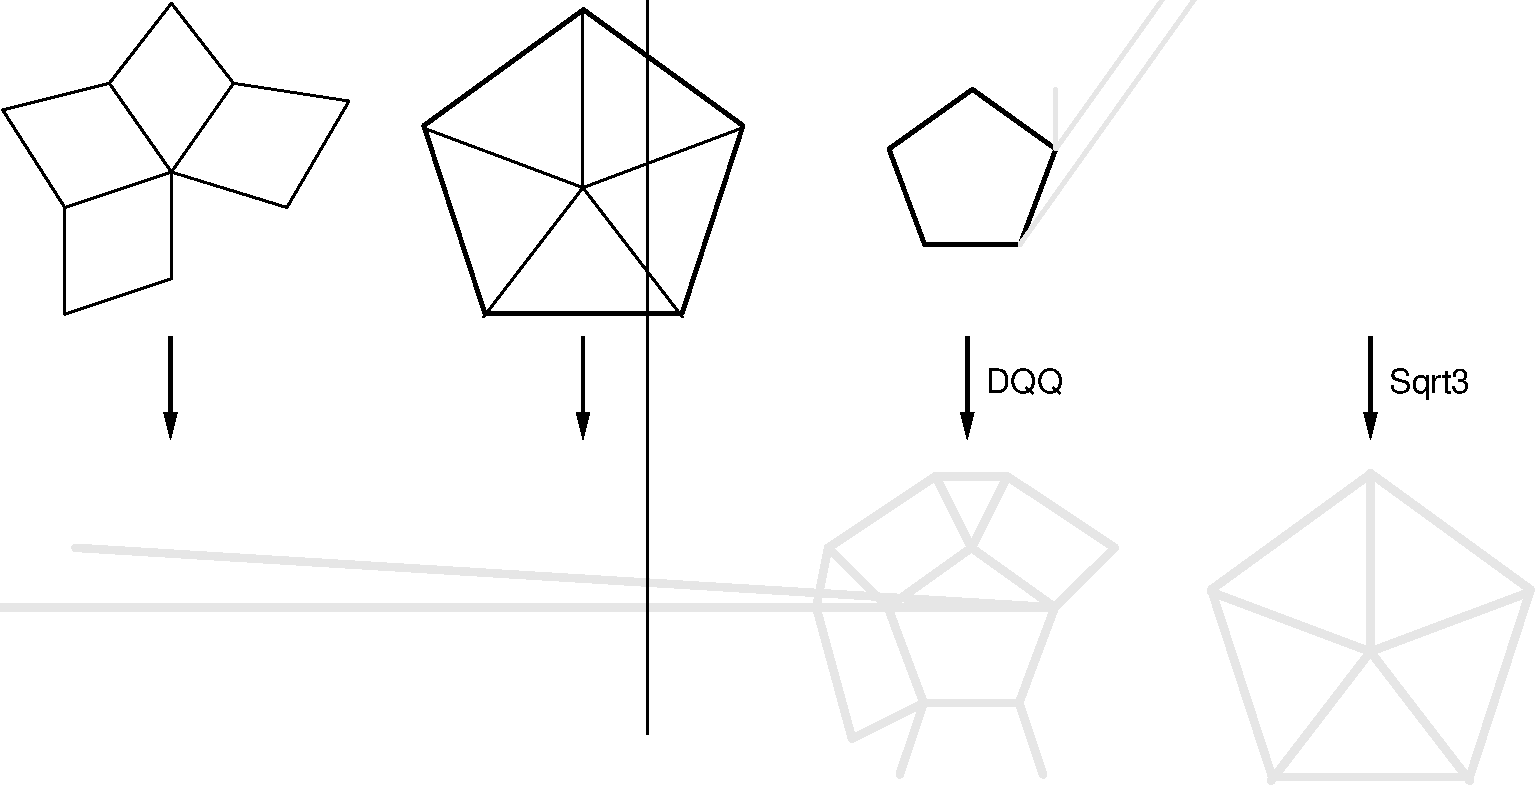
\includegraphics[width=0.6\textwidth]{Subdivision_method_3/FIG/RefSchemes}%
    }\\ \vspace{0.5cm}
  \end{center}
\end{ccTexOnly}

\begin{ccHtmlOnly}
  <CENTER>
     <img src="FIG/RefSchemes.gif" alt="Refinement Hosts"><P>
  </CENTER>
\end{ccHtmlOnly}

The figure demonstrates these four refinement patterns on 
the 1-disk of a valence-5 vertex/facet.
Refined meshes are shown below the source meshes. 
%We call a source mesh \emph{control mesh} if it is
%the origin of a squence of refinements.
Points on the refined mesh are generated by averaging
neighbor points on the source mesh. A graph, called \emph{stencil}, 
determines the source neighborhood whose points contribute to the 
position of a refined point. A refinement pattern usually defines 
more than one stencil.
%Stencils are defined at the time the refinement pattern is chosen.  
%as illustrated in Figure \ref{fig:RefMap},
For example, the PQQ
%\emph{P}rimal \emph{Q}uadtrateral \emph{Q}uadrisection (PQQ) scheme 
refinement has a vertex-node stencil, 
which defines the 1-ring of an input vertex; an edge-node stencil, 
which defines the 1-ring of an input edge; and a facet-node stencil, 
which defines an input facet. The stencils of the PQQ refinement are
shown in the following figure. The blue neighborhoods in the 
top row indicate the corresponding stencils of the refined nodes 
in red. 

\begin{ccTexOnly}
  \begin{center}
    \parbox{0.5\textwidth}{%
      
\includegraphics[width=0.5\textwidth]{Subdivision_method_3/FIG/PQQStencil}%
    }\\ \vspace{0.5cm}
  \end{center}
\end{ccTexOnly}

\begin{ccHtmlOnly}
  <CENTER>
     <img src="FIG/PQQStencil.gif" alt="Stencils of PQQ scheme "><P>
  </CENTER>
\end{ccHtmlOnly}


%while the DQQ scheme has only a corner-node stencil, which 
%relates the facet of a corner to a target node.
Stencils with weights are called \emph{geometry masks}.
%One practical set of geometry masks of the PQQ scheme is
A subdivision method defines a geometry mask for each stencil, and 
generates new points by averaging source points weighted by the mask.
Geometry masks are carefully chosen to meet requirements of 
certain surface smoothness and shape quality.
The geometry masks of Catmull-Clark subdivision are shown
below.  

\begin{ccTexOnly}
  \begin{center}
    \parbox{0.4\textwidth}{%
      
\includegraphics[width=0.4\textwidth]{Subdivision_method_3/FIG/cc_mask}%
    } \\ \vspace{0.5cm}
  \end{center}
\end{ccTexOnly}

\begin{ccHtmlOnly}
  <CENTER>
     <img src="FIG/cc_mask.gif" alt="Catmull-Clark geometry stencil"><P>
  </CENTER>
\end{ccHtmlOnly}

The weights shown here are unnormalized, and $n$ is the valence 
of the vertex. The generated point, in red, is computed by a summation
of the weighted points. For example, a Catmull-Clark facet-node is 
computed by the summation of $1/4$ of each point on its stencil.

A stencil can have an unlimited number of geometry masks. For example, 
a facet-node of PQQ refinement may be computed by 
the summation of $1/5$ of each stencil node instead of $1/4$.
Although it is legal in \ccc{Subdivision_method_3} to have 
any kind of geometry mask, the result surfaces may be odd, 
not smooth, or not even exist. \cite{cgal:ww-smgd-02} explains the 
details on designing masks for a quality subdivision surface.

%The averaging process can typically be factored into 
%simpler steps \cite{Oswald-2003-CSS}.
%and this has been implemented in the OpenMesh library \cite{Sovakar-2004-APISUB}.
%However, while stencil factoring simplifies the implementation,
%it is less efficient because it requires repeated visits 
%to all nodes.

%% Since only a fixed number of refinement patterns are 
%% practical but a wide variety of geometry masks can be developed,
%% \ccc{Subdivision_method_3} provides a set of refinement patterns 
%% (the \emph{refinement hosts})
%% and hands the definition of geometry masks
%% (the \emph{geometry policies}) to the library user.
%% A subdivision scheme is obtained by parameterizing the 
%% refinement host with geometry policies. 
%% For example, Catmull-Clark subdivision is constructed by 
%% parameterizing the PQQ refinement with the Catmull-Clark geometry 
%% policies.

%, which compute the smoothed points based on the
%Catmull-Clark geometry masks.

%A subdivision scheme of \ccc{CGAL::Subdivision_method_3} is a 
%refinement host parameterized with a geometry policy. 

%The refinement host realizes the topological refinement and 
%the stencils. The geometry policy consists a set of 
%averaging rules of the geometry stencils.

% +-------------------------------------------------------------+
\section{A Quick Example: Catmull-Clark Subdivision}
\label{secFirstSub}
Assuming you are familiar with \ccc{Polyhedron_3},
you can integrate \ccc{Subdivision_method_3} into your program 
without much effort.

\ccIncludeExampleCode{Subdivision_method_3/CatmullClark_subdivision.C}

This example demonstrates the use of the Catmull-Clark subdivision method
on a \ccc{Polyhedron_3}. The polyhedron is restricted in the Cartesian
space, where most subdivision applications are designed to work.
There is only one line deserving a detailed explanation:
\begin{ccExampleCode}
Subdivision_method_3::CatmullClark_subdivision(P,d);
\end{ccExampleCode}
\ccc{Subdivision_method_3} specifies the namespace of our
subdivision functions. \ccc{CatmullClark_subdivision(P,d)} computes the 
Catmull-Clark subdivision surface of the polyhedron \ccc{P} after
\ccc{d} iterations of the refinements. The polyhedron \ccc{P} is 
passed by reference, and is modified (i.e.~subdivided) by the 
subdivision function.

%Other subdivision methods (such as Doo-Sabin subdivision) can be
%used with the same level of the ease.

This example shows how to subdivide a simple \ccc{Polyhedron_3}
with \ccc{Subdivision_method_3}.
An application-defined polyhedron might use a specialized kernel and/or
a specialized internal container. There are two major restrictions on the 
application-defined polyhedron to work with 
\ccc{Subdivision_method_3}.
\begin{itemize}
\item
\ccc{Point_3} is type-defined by the kernel. Without \ccc{Point_3} 
and the associated operations being defined, \ccc{Subdivision_method_3} 
can not know how to compute and store the new vertex points.
\item
The primitives (such as vertices, halfedges and facets) 
in the internal container are sequentially ordered (e.g.~
\ccc{std::vector} and \ccc{std::list}).
This implies that the iterators traverse the primitives in 
the order of their creations/insertions.
\end{itemize}

Section~\ref{secRefHost} gives detailed explanations on those 
two restrictions.

% +-------------------------------------------------------------+
\section{Catmull-Clark Subdivision}
\label{secCC}
%\ccc{Subdivision_method_3} provides direct functions on 
%Catmull-Clark, Loop, Doo-Sabin and $\sqrt{3}$ subdivision methods.
\ccc{Subdivision_method_3} is designed to allow customization of 
the subdivision methods. This section explains the implementation
of the Catmull-Clark subdivision function in \ccc{Subdivision_method_3}.
The implementation demonstrates the customization of the PQQ refinement 
to Catmull-Clark subdivision. 

When a subdivision method is developed, a refinement pattern is 
chosen, and then a set of geometry masks are developed to 
position the new points. There are three key components 
to implement a subdivision method: 
\begin{itemize}
\item
a mesh data structure that can represent arbitrary 2-manifolds, 
\item
a process that refines the mesh data structure, 
\item
and the geometry masks that compute the new points.
\end{itemize}

E. Catmull and J. Clark picked the
PQQ refinement for their subdivision method,
and developed a set of geometry masks to generate (or more 
precisely, to approximate) the B-spline surface from 
the control mesh.
\ccc{Subdivision_method_3} provides a function that glues all 
three components of the Catmull-Clark subdivision method.

\begin{ccExampleCode}
template <class Polyhedron_3, template <typename> class Mask>
void PQQ(Polyhedron_3& p, Mask<Polyhedron_3> mask, int depth)
\end{ccExampleCode}

\ccc{Polyhedron_3} is a generic mesh data structure for 
arbitrary 2-manifolds. \ccc{PQQ()}, the \emph{refinement host},
provides the process refining the control mesh \ccc{p}. 
During the refinement, \ccc{PQQ()} computes and assigns
new points by cooperating with the \ccc{mask}. 
To implement Catmull-Clark subdivision,
\ccc{Mask}, the \emph{geometry policy}, has to realize the 
geometry masks of Catmull-Clark subdivision. 
\ccc{depth} specifies the iterations of the refinement 
on the control mesh. 
%To make the call to
%\ccc{PQQ} a Catmull-Clark subdivision, the only thing left is to
%implement a geometry policy realizing the Catmull-Clark geometry masks.

To implement the geometry masks, we need to know how  
a refinement host communicates with its geometry masks. 
The PQQ refinement defines three stencils, and hence 
three geometry masks are required for Catmull-Clark subdivision.
The following class defines the interfaces of the stencils 
for the PQQ refinement.

\begin{ccExampleCode}
template <class Polyhedron_3>
class PQQ_stencil_3 {
  void facet_node(Facet_handle facet, Point_3& pt);
  void edge_node(Halfedge_handle edge, Point_3& pt);
  void vertex_node(Vertex_handle vertex, Point_3& pt);
};
\end{ccExampleCode}

Each class function in \ccc{PQQ_stencil_3} 
computes a new point based on the neighborhood of the primitive 
handle, and assigns the new point to \ccc{Point_3& pt}. 

We realize each class function with the geometry masks of 
Catmull-Clark subdivision. 

\begin{ccExampleCode}
template <class Polyhedron_3>
class CatmullClark_mask_3 {
  void facet_node(Facet_handle facet, Point_3& pt) {
    Halfedge_around_facet_circulator hcir = facet->facet_begin();
    int n = 0;
    Point_3 p(0,0,0);
    do {
      p = p + (hcir->vertex()->point() - ORIGIN);
      ++n;
    } while (++hcir != facet->facet_begin());
    pt = ORIGIN + (p - ORIGIN)/FT(n);
  }
  void edge_node(Halfedge_handle edge, Point_3& pt) {
    Point_3 p1 = edge->vertex()->point();
    Point_3 p2 = edge->opposite()->vertex()->point();
    Point_3 f1, f2;
    facet_node(edge->facet(), f1);
    facet_node(edge->opposite()->facet(), f2);
    pt = Point_3((p1[0]+p2[0]+f1[0]+f2[0])/4,
                 (p1[1]+p2[1]+f1[1]+f2[1])/4,
                 (p1[2]+p2[2]+f1[2]+f2[2])/4 );
  }
  void vertex_node(Vertex_handle vertex, Point_3& pt) {
    Halfedge_around_vertex_circulator vcir = vertex->vertex_begin();
    int n = circulator_size(vcir);    

    FT Q[] = {0.0, 0.0, 0.0}, R[] = {0.0, 0.0, 0.0};
    Point_3& S = vertex->point();
    
    Point_3 q;
    for (int i = 0; i < n; i++, ++vcir) {
      Point_3& p2 = vcir->opposite()->vertex()->point();
      R[0] += (S[0]+p2[0])/2;
      R[1] += (S[1]+p2[1])/2;
      R[2] += (S[2]+p2[2])/2;
      facet_node(vcir->facet(), q);
      Q[0] += q[0];      
      Q[1] += q[1];      
      Q[2] += q[2];
    }
    R[0] /= n;    R[1] /= n;    R[2] /= n;
    Q[0] /= n;    Q[1] /= n;    Q[2] /= n;
      
    pt = Point_3((Q[0] + 2*R[0] + S[0]*(n-3))/n,
                 (Q[1] + 2*R[1] + S[1]*(n-3))/n,
                 (Q[2] + 2*R[2] + S[2]*(n-3))/n );
  }
};
\end{ccExampleCode}

This example shows the default implementation of Catmull-Clark 
masks in \ccc{Subdivision_method_3}.
This default implementation assumes the \emph{types} 
(such as \ccc{Point_3} and \ccc{Facet_handle}) are defined 
within \ccc{Polyhedron_3}. \ccc{CatmullClark_mask_3} 
is designed to work on a \ccc{Polyhedron_3} with the \ccc{Cartesian} 
kernel. You may need to rewrite the geometry computation
to match the kernel geometry of your application.

To invoke the Catmull-Clark subdivision method, we
call \ccc{PQQ()} with the Catmull-Clark masks we just defined.

\begin{ccExampleCode}
PQQ(p, CatmullClark_mask_3<Polyhedron_3>(), depth);
\end{ccExampleCode}

%\begin{ccExampleCode}
%template <class Polyhedron_3>
%void CatmullClark_subdivision(Polyhedron_3& p, int depth) {
%    PQQ(p, CatmullClark_mask_3<Polyhedron_3>(), depth);
%}
%\end{ccExampleCode}

Loop, Doo-Sabin and $\sqrt{3}$ subdivisions are implemented 
in the similar process: pick a refinement host and implement 
the geometry policy. The key of developing your own 
subdivision method is implementing the right combination of 
the refinement host and the geometry policy. It is 
explained in the next two sections.

% +-------------------------------------------------------------+
\section{Refinement Host}
\label{secRefHost}
A refinement host is a template function of 
a polyhedron class and a geometry mask class. It refines
the input polyhedron, and computes new points through the geometry masks.
\ccc{Subdivision_method_3} supports four refinement hosts:
primal quadrilateral quadrisection (PQQ), 
primal triangle quadrisection (PTQ), dual quadrilateral 
quadrisection (DQQ) and $\sqrt{3}$ triangulation.
Respectively, they are used by Catmull-Clark, Loop, Doo-Sabin 
and $\sqrt{3}$ subdivision. 

\begin{ccTexOnly}
  \begin{center}
    \parbox{0.6\textwidth}{%
      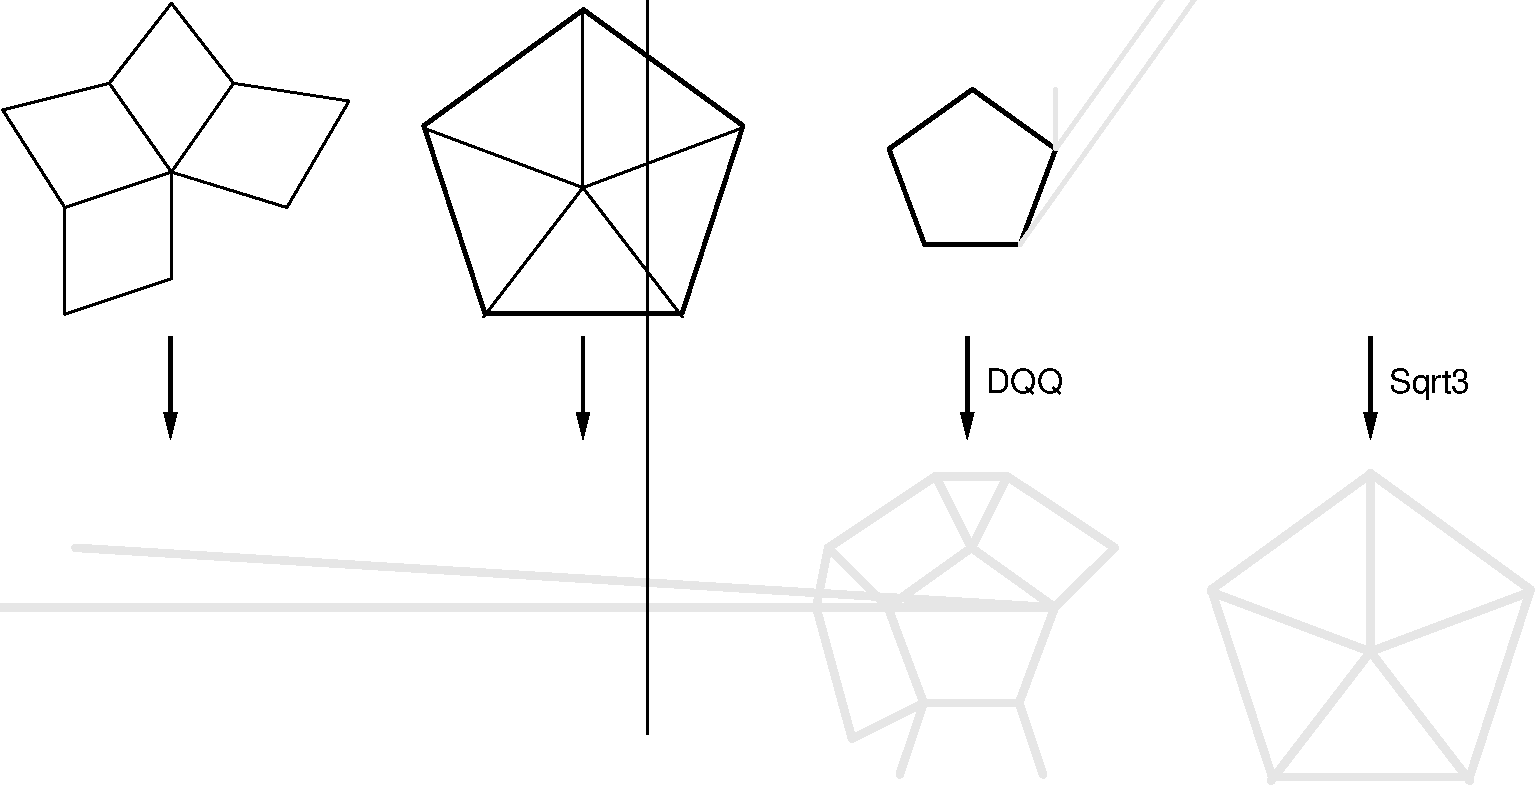
\includegraphics[width=0.6\textwidth]{Subdivision_method_3/FIG/RefSchemes}%
    }\\ \vspace{0.5cm}
%    \ccc{Subdivision_method_3} supports hosts of these four refinement 
%    schemes that are demonstrated on a valence-n submesh.
%    The refined mesh is shown below the control mesh.
  \end{center}
\end{ccTexOnly}

\begin{ccHtmlOnly}
  <CENTER>
     <img src="FIG/RefSchemes.gif" alt="Refinement Hosts"><P>
  </CENTER>
\end{ccHtmlOnly}


\begin{ccExampleCode}
namespace Subdivision_method_3 {
  template <class Polyhedron_3, template <typename> class Mask>
  void PQQ(Polyhedron_3& p, Mask<Polyhedron_3> mask, int step);

  template <class Polyhedron_3, template <typename> class Mask>
  void PTQ(Polyhedron_3& p, Mask<Polyhedron_3> mask, int step);

  template <class Polyhedron_3, template <typename> class Mask>
  void DQQ(Polyhedron_3& p, Mask<Polyhedron_3> mask, int step)

  template <class Polyhedron_3, template <typename> class Mask>
  void Sqrt3(Polyhedron_3& p, Mask<Polyhedron_3> mask, int step)
}
\end{ccExampleCode}

%% Stencils are maintained using the iteration concept
%% to avoid the need for vertex tags to distinguish
%% the stencil types.
%% For example, on a PQQ refined mesh, the vertex iterator 
%% visits the 
%% vertex-nodes, edge-nodes and then facet-nodes. The visit
%% order is implicitly used to determine the stencil of
%% the visited node.

The polyhedron class is a specialization of
\ccc{Polyhedron_3}, and the mask is a policy 
class realizing the geometry masks of the subdivision 
method.

A refinement host refines the input polyhedron, maintains 
the stencils (i.e., the mapping between the control mesh 
and the refined mesh), and calls the geometry masks
to compute the new points. 
In \ccc{Subdivision_method_3}, refinements are implemented
as a sequence of connectivity operations (mainly Euler operations).
The order of the connectivity operations plays a key role when maintaining
stencils. By matching the order of the source submeshes to the refined 
vertices, no flag in the primitives is required to register the stencils. 
It avoids the data dependency of the refinement host on the polyhedron class. 
To make the ordering trick work, the polyhedron class must 
have a sequential container, such as a vector or a linked-list, as
the internal storage. 
%The polyhedron class always inserts
%new primitives at the end, and 
A sequential container guarantees that the iterators of the 
polyhedron always traverse the primitives in the order of their 
insertions. Non-sequential structures such as 
trees or maps do not provide the required ordering, and hence
can not be used with \ccc{Subdivision_method_3}.
 
Although \ccc{Subdivision_method_3} does not require flags
to support the refinements and the stencils, it
still needs to know how to compute and store the geometry
data (i.e.~the points). \ccc{Subdivision_method_3} 
expects that the typename \ccc{Point_3} is 
defined in the geometry kernel of the polyhedron
(i.e.~the \ccc{Polyhedron_3::Traits::Kernel}). 
A point of the type \ccc{Point_3} is returned by the geometry 
policy and is then assigned to the new vertex.  
The geometry policy is explained in next section. 

Refinement hosts \ccc{PQQ} and \ccc{DQQ} work on a general 
polyhedron, and \ccc{PTQ} and \ccc{Sqrt3} work on a triangulated
polyhedron. The result of \ccc{PTQ} and \ccc{Sqrt3} on a non-triangulated
polyhedron is undefined. \ccc{Subdivision_method_3} does not verify
the precondition of the mesh characteristics before the refinement.

For details of the refinement implementation, 
interested users should refer to \cite{cgal:sp-mrbee-05}.

% +-------------------------------------------------------------+
\section{Geometry Policy}
A geometry policy defines a set of geometry masks. 
Each geometry mask is realized as a member function
that computes new points of the subdivision surface. 
%The policy interface is defined with the refinement host. 

Each geometry mask receives a primitive handle 
(e.g.~\ccc{Halfedge_handle}) of the control mesh, 
and returns a \ccc{Point_3} to the subdivided vertex. 
The function collects the vertex neighbors of the primitive handle 
(i.e.~nodes on the stencil), and computes the new point 
based on the neighbors and the mask (i.e.~the stencil weights).

\begin{ccTexOnly}
  \begin{center}
    \parbox{0.4\textwidth}{%
      
\includegraphics[width=0.4\textwidth]{Subdivision_method_3/FIG/cc_mask}%
    } \\ \vspace{0.5cm}
  \end{center}
\end{ccTexOnly}
\begin{ccHtmlOnly}
  <CENTER>
     <img src="FIG/cc_mask.gif" alt="Catmull-Clark geometry stencil"><P>
  </CENTER>
\end{ccHtmlOnly}

This figure shows the geometry masks of
Catmull-Clark subdivision. The weights shown here are unnormalized, 
and $n$ is the valence of the vertex. The new points are 
computed by the summation of the weighted points on their stencils.
Following codes show an implementation of the geometry mask of 
the facet-node. The complete listing
of a Catmull-Clark geometry policy is in the Section~\ref{secCC}.

\begin{ccExampleCode}
template <class Polyhedron_3>
class CatmullClark_mask_3 {
  void facet_node(Facet_handle facet, Point_3& pt) {
    Halfedge_around_facet_circulator hcir = facet->facet_begin();
    int n = 0;
    Point_3 p(0,0,0);
    do {
      p = p + (hcir->vertex()->point() - ORIGIN);
      ++n;
    } while (++hcir != facet->facet_begin());
    pt = ORIGIN + (p - ORIGIN)/FT(n);
  }
}
\end{ccExampleCode}

In this example, the computation is based on the assumption that
the \ccc{Point_3} is the \ccc{CGAL::Point_3}. It is an assumption, 
but not a restriction.
You are allowed to use any point class as long as it is
defined as the \ccc{Point_3} in your polyhedron.
You may need to modify the geometry policy to support the computation
and the assignment of the specialized point. This extension is not unusual 
in graphics applications. For example, you might want to subdivide the
texture coordinates for your subdivision surface. 
%The typename 
%\ccc{Point_3} is actually the attribute holder, including the 
%point of course, for the vertices.

The refinement host of Catmull-Clark subdivision
requires three geometry masks for 
polyhedrons without open boundaries: a vertex-node 
mask, an edge-node mask, and a facet-node mask. 
To support polyhedrons with boundaries, a border-node mask is 
also required. The border-node mask for Catmull-Clark subdivision
is listed below, where \ccc{ept} returns the new point splitting 
\ccc{edge} and \ccc{vpt} returns the new point on the vertex pointed by
\ccc{edge}.  

%% \begin{ccTexOnly}
%%   \begin{center}
%%     \parbox{0.5\textwidth}{%
%%       
\includegraphics[width=0.5\textwidth]{Subdivision_method_3/FIG/PQQStencil}%
%%     }
%%   \end{center}
%% \end{ccTexOnly}

\begin{ccExampleCode}
  void border_node(Halfedge_handle edge, Point_3& ept, Point_3& vpt) {
    Point_3& ep1 = edge->vertex()->point();
    Point_3& ep2 = edge->opposite()->vertex()->point();
    ept = Point_3((ep1[0]+ep2[0])/2, (ep1[1]+ep2[1])/2, (ep1[2]+ep2[2])/2);

    Halfedge_around_vertex_circulator vcir = edge->vertex_begin();
    Point_3& vp1  = vcir->opposite()->vertex()->point();
    Point_3& vp0  = vcir->vertex()->point();
    Point_3& vp_1 = (--vcir)->opposite()->vertex()->point();
    vpt = Point_3((vp_1[0] + 6*vp0[0] + vp1[0])/8,
                  (vp_1[1] + 6*vp0[1] + vp1[1])/8,
                  (vp_1[2] + 6*vp0[2] + vp1[2])/8 );
  }
\end{ccExampleCode}


The mask interfaces of all four refinement hosts are listed below.
\ccc{DQQ_stencil_3} and \ccc{Sqrt3_stencil_3} 
do not have the border-node stencil because the refinement hosts of
DQQ and $\sqrt{3}$ refinements do not support global boundaries in the 
current release. This might be changed in the future releases.

%The interface of a geometry policy need to match the stencils of 
%the refinement host. We have already seen the geometry masks for
%a PQQ-base subdivision, Catmull-Clark subdivision. 
%The mask interface the other three refinement hosts, PTQ, DQQ and 
%$\sqrt{3}$, are defined below 
%(PQQ as well).


\begin{ccExampleCode}
template <class Polyhedron_3>
class PQQ_stencil_3 {
  void facet_node(Facet_handle, Point_3&);
  void edge_node(Halfedge_handle, Point_3&);
  void vertex_node(Vertex_handle, Point_3&);

  void border_node(Halfedge_handle, Point_3&, Point_3&);
};

template <class Polyhedron_3>
class PTQ_stencil_3 {
  void edge_node(Halfedge_handle, Point_3&);
  void vertex_node(Vertex_handle, Point_3&);

  void border_node(Halfedge_handle, Point_3&, Point_&);
};

template <class Polyhedron_3>
class DQQ_stencil_3 {
public:
  void corner_node(Halfedge_handle edge, Point_3& pt);
};

template <class Polyhedron_3>
class Sqrt3_stencil_3 {
public:
  void vertex_node(Vertex_handle vertex, Point_3& pt);
};
\end{ccExampleCode}

The source codes of \ccc{CatmullClark_mask_3}, \ccc{Loop_mask_3},
\ccc{DooSabin_mask_3}, and \ccc{Sqrt3_mask_3} are
the best sources of learning these stencil interfaces. 


%Note, only the \ccc{PQQ_stencil_3} and the \ccc{DQQ_stencil_3}
%are provided in \ccc{Subdivision_method_3}.
%The \ccc{PTQ_stencil_3} and the \ccc{Sqrt3_stencil_3} are given
%here for reference only. Both stencils are a subset of the
%\ccc{PQQ_stencil_3}, and you can just use the 
%\ccc{PQQ_stencil_3} to develop masks for PTQ or $\sqrt{3}$ 
%schemes. 


%% \begin{ccExampleCode}
%% PQQ<_M,CCstencil>(Mesh,CCstencil<_M>())
%% \end{ccExampleCode}
%% (or, more simply \\
%% \begin{ccExampleCode}
%% PQQ(Mesh,CCstencil<_M>())}
%% \end{ccExampleCode}
%% since the compiler can derive the template
%% arguments from the function parameters),
%% instantiates Catmull-Clark subdivision.    
%% \ccc{_M}, the model of the mesh concept,
%% represents the mesh type (\ccc{Mesh}),
%% and \ccc{CCstencil} is a class template 
%% realizing geometry policies of Catmull-Clark subdivision.

%The geometry stencils of Catmull-Clark subdivision (border stencils are 
%not included) are shown below. 

%\begin{ccTexOnly}
%  \begin{center}
%    \parbox{0.4\textwidth}{%
%      
\includegraphics[width=0.4\textwidth]{Subdivision_method_3/FIG/cc_mask}%
%    }
%  \end{center}
%\end{ccTexOnly}

%\begin{ccHtmlOnly}
%  <CENTER>
%  <A HREF="FIG/cc_mask.gif">
%     <img src="FIG/cc_mask.gif" alt="Catmull-Clark geometry stencil"></A><P>
%  </CENTER>
%\end{ccHtmlOnly}


% +------------------------------------------------------------------------+
\section{The Four Subdivision Methods}
% +------------------------------------------------------------------------+
\ccc{Subdivision_method_3} supports Catmull-Clark, Loop, 
Doo-Sabin and $\sqrt{3}$ subdivisions by specializing
their respective refinement hosts. 
%The hosts are specialized with
%the geometry masks we introduced in th previous sections. 
They are designed to work on a \ccc{Polyhedron_3}. If your application 
uses a polyhedron with a specialized geometry kernel, you need to 
specialize the refinement host with a geometry policy 
based on that kernel.

\begin{ccExampleCode}
namespace Subdivision_method_3 {
  template <class Polyhedron_3>
  void CatmullClark_subdivision(Polyhedron_3& p, int step = 1) {
    PQQ(p, CatmullClark_mask_3<Polyhedron_3>(), step);
  }

  template <class Polyhedron_3>
  void Loop_subdivision(Polyhedron_3& p, int step = 1) {
    PTQ(p, Loop_mask_3<Polyhedron_3>() , step);
  }

  template <class Polyhedron_3>
  void DooSabin_subdivision(Polyhedron_3& p, int step = 1) {
    DQQ(p, DooSabin_mask_3<Polyhedron_3>(), step);
  }

  template <class Polyhedron_3>
  void Sqrt3_subdivision(Polyhedron_3& p, int step = 1) {
    Sqrt3(p, Sqrt3_mask_3<Polyhedron_3>(), step);
  }
}
\end{ccExampleCode}

The following example demonstrates the use of Doo-Sabin subdivision 
on a polyhedral mesh.
\ccIncludeExampleCode{Subdivision_method_3/DooSabin_subdivision.C}

% +------------------------------------------------------------------------+
\section{Other Subdivision Methods}
% +------------------------------------------------------------------------+
\ccc{Subdivision_method_3} supports four practical subdivision methods on a
Cartesian \ccc{Polyhedron_3}. More subdivision methods can be supported
through the specialization of refinement hosts with custom geometry masks. 
The following example develops a subdivision method 
generating an improved Loop subdivision surface. 
%Loop subdivision is
%based on the PTQ refinement. The geometry policy is developed as a subclass 
%of \ccc{PQQ_stencil_3}, which defines the superset of PTQ stencils.

\ccIncludeExampleCode{Subdivision_method_3/Customized_subdivision.C}

The points generated by the geometry mask are semantically
required to converge to a smooth surface. This is the requirement
imposed by the theory of the subdivision surface.
\ccc{Subdivision_method_3} does not enforce this requirement, nor will
it verify the smoothness of the subdivided mesh. 
\ccc{Subdivision_method_3} guarantees the topological properties of 
the subdivided mesh. A genus-$n$ 2-manifold is assured to be subdivided
into a genus-$n$ 2-manifold. But when specialized with ill-designed
geometry masks, \ccc{Subdivision_method_3} may generate a surface that is 
odd, not smooth, or not even exist.


